\documentclass[12pt,a4paper]{article}
\usepackage[utf8]{inputenc}
\usepackage[german]{babel}
\usepackage[T1]{fontenc}
\usepackage{amsmath}
\usepackage{amsfonts}
\usepackage{amssymb}
\usepackage{graphicx}
\usepackage[left=2.5cm,right=2.5cm,top=2cm,bottom=2cm]{geometry}
\usepackage{float}
\author{Gruppe C14 \\ Julián Häck, Martin Koytek, Lars Wenning, Erik Zimmermann}
\begin{document}
\section{Charakterisieren eines Kondensators}
\subsection{Versuchsbeschreibung}
In diesem Teil des Versuchs werden wir uns im speziellen die Lade- bzw. Entladekurven des Kondensators anschauen, um diesen zu bestimmen. Wir werden danach in Python die Daten auswerten, logarithmisch fitten und so beim Aufladevorgang die Kapazität C (in $\mu$F) über den Verlauf der Stromstärke, sowie beim Entladevorgang über den Spannungsverlauf bestimmen. Wir werden unsere Ergebnisse anhand von Residuenplots evaluieren.\\
\subsection{Versuchsaufbau und Durchführung}
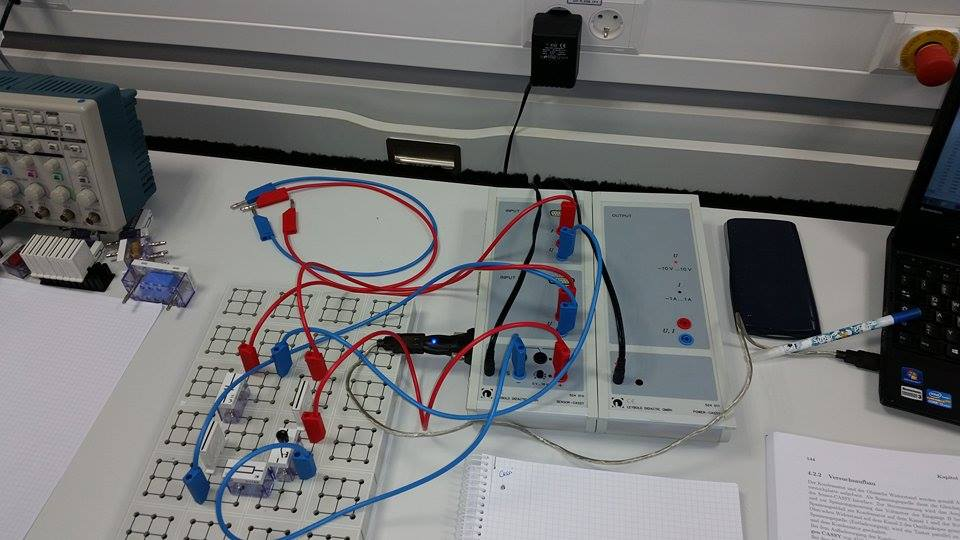
\includegraphics[scale=0.35]{12834837_1207198225971904_686312351_n.jpg}
\\Oben sieht man unseren Versuchsaufbau. Dieser unterscheidet sich prinzipiell nicht vom Aufbau bei der Messung mit dem Oszilloskop. Wir greifen immer noch parallel zum Kondensator die Spannung ab, sowie in Reihe die Stromstärke. Ein Schalter unterbricht den Stromkreis und löst so den Lade- bzw. Entladevorgang aus.\\
\\Unser Messbereich im Cassy liegt für die Spannung bei 10V und bei der Stromstärke 0.1A. Wir verwenden einen 1k$\Omega$ Widerstand um den Lade- und Entladevorgang zu verzögern. Des Weiteren verwenden wir einen 1$\mu$F Kondensator den wir im Experiment charakterisieren möchten.\\
Als Trigger benutzen wir die eingebaute Cassy-Funktion und triggern jeweils die Spannung (0.4V beim Ladevorgang, 7.6V beim Entladevorgang).\\
Wir verwenden die höchstmögliche Messauflösung von 10$\mu$s und 10ms Messzeit.\\
\\Beim Ladevorgang stellen wir die automatische Umschaltfunktion der Spannungsquelle (8V Ladespannung) des Cassy an und starten dann die Messung. Wir messen sowohl die Stromstärke, als auch die Spannung, betrachten aber später aufgrund ihrer Form beim Ladevorgang nur den Verlauf der Stromstärke. Wir messen insgesamt 4 Ladevorgänge, um später den Kondensator genauer bestimmen zu können. \\
\\Beim Entladevorgang schalten wir die Spannungsquelle von vornherein an, warten ab bis sich die Ladespannung von 8V eingestellt hat und triggern jetzt den Abfall der Spannung. Den Trigger lösen wir durch kurzschließen der Spannungsquelle aus. Der dabei gemessene Spannungsverlauf wird dann später ausgewertet. Auch hier messen wir wieder 4 mal, um unsere Genauigkeit zu erhöhen.\\
\subsection{Versuchsauswertung}
\subsubsection{Rohdaten}
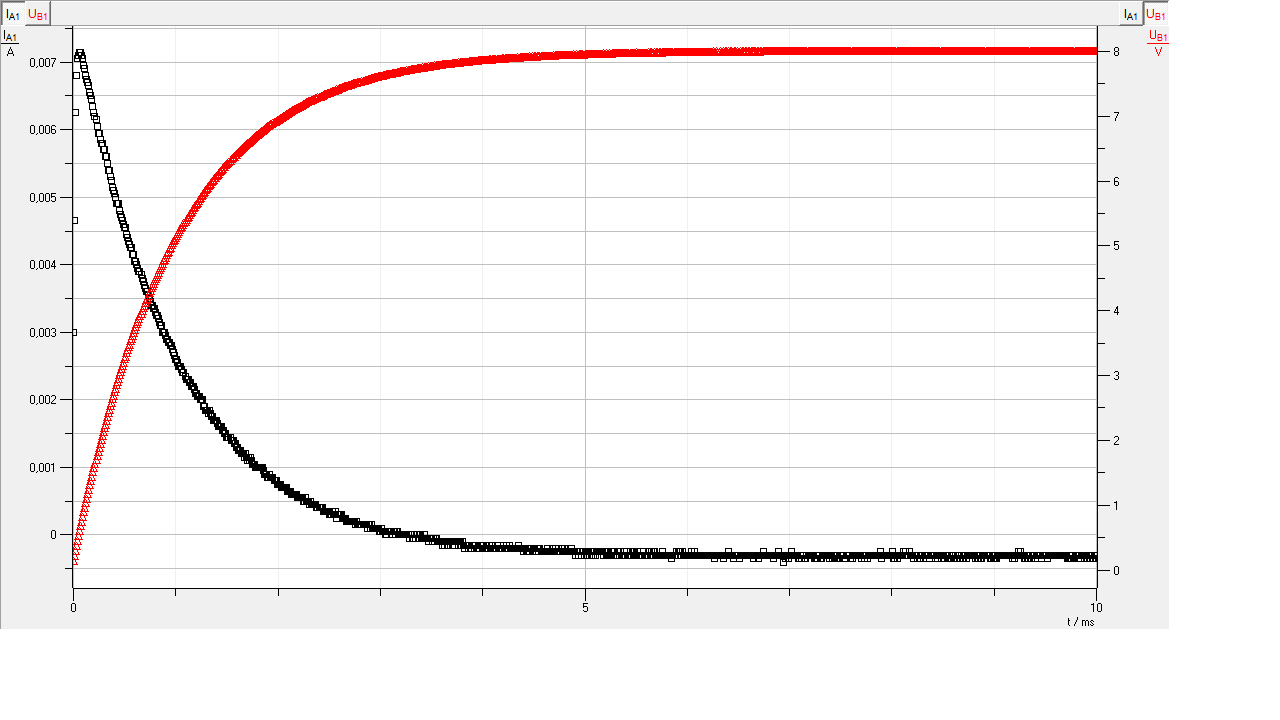
\includegraphics[scale=0.35]{auf1.png}\\
Aufladevorgang (U in V [rot], I in A [schwarz]gegen t in ms)\\
\\
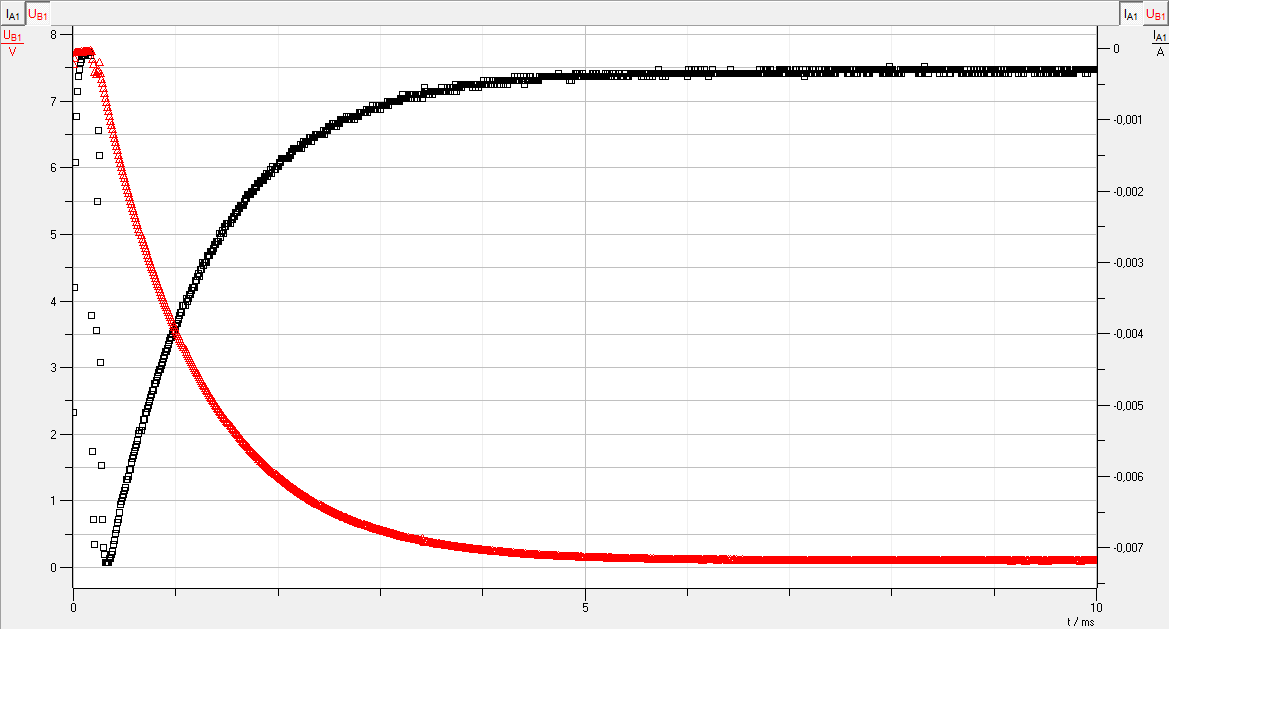
\includegraphics[scale=0.35]{ent1.png}\\
Entladevorgang (U in V [rot], I in A [schwarz]gegen t in ms)\\

\subsubsection{Transformation der Rohdaten}
Um an den oben aufgeführten Daten eine lineare Regression durchführen zu können müssen wir die Datenpunkte logarithmieren. Wie bereits vorher angekündigt verwenden wir beim Ladevorgang nur die Daten der Stromstärkenmessung und beim Entladevorgang die Daten der Spannungsmessung. Im Folgenden werden wir das jeweils anhand eines Beispieles für Spannung und Stromstärke zeigen, da der Bericht sonst zu lang wird. In unseren Endwerten sind alle Daten mit eingearbeitet, um ein möglichst genaues Ergebnis zu erzielen.\\
\\Bevor wir anfangen die Daten zu logarithmieren, müssen wir die Offsets bestimmen. Dies machen wir grafisch in Cassy.\\
Dazu zoomen wir auf den $\,$geraden$\,$ Bereich der abfallenden e-Funktion am Ende der Messung. Wenn wir nur noch Rauschen und keinen signifikanten Abfall der Werte sehen, können wir den untersten Peak mit einer Einheit in der Größenordnung darunter als Offset bestimmen. In dieser Ansicht können wir auch die Auflösung der Spannung bzw. Stromstärke ablesen, aus der wir die gleichverteilte Unsicherheit auf unsere Messwerte ablesen. Wir verfahren ähnlich mit der Zeitskala und bei den anderen Messungen.\\
\\
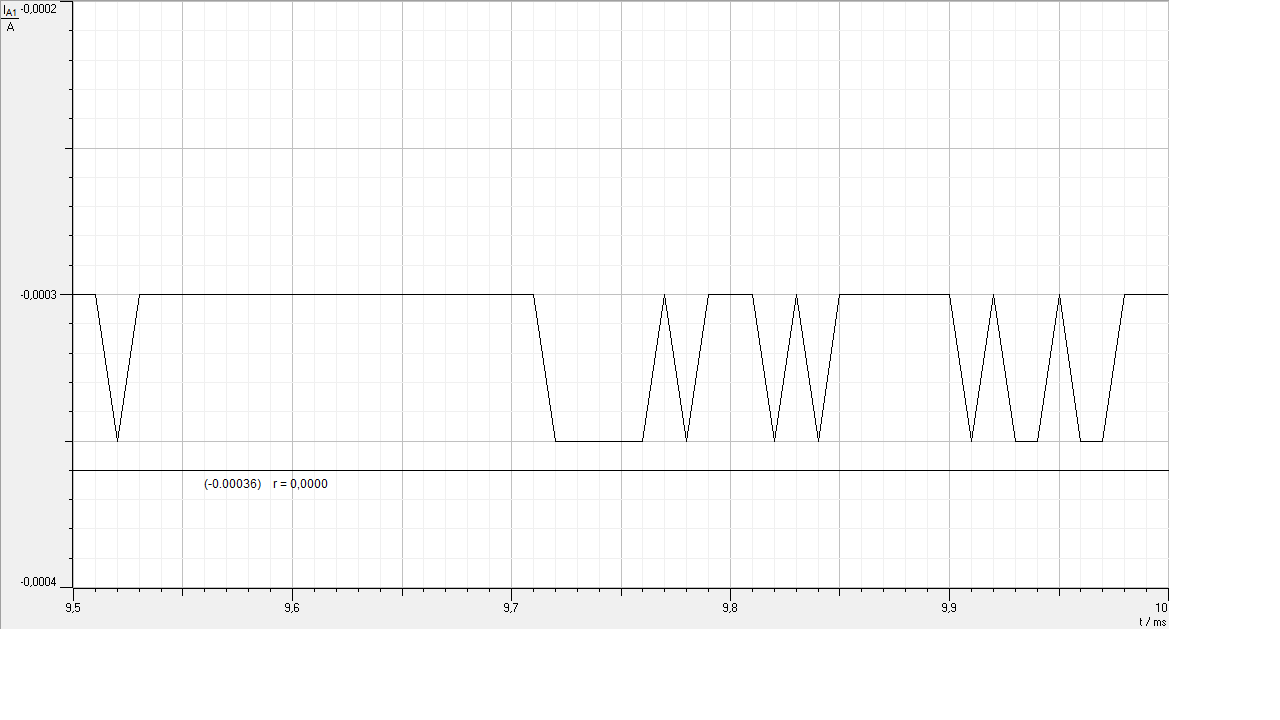
\includegraphics[scale=0.35]{offset_und_fehler.png}\\
Unterer Bereich des Ladevorgangs (I in A gegen t in ms) und Offsetmarkierung\\
\\
\\In unserem Beispiel haben wir nun einen Offset bei der Aufladung von -0.00041 A, einen Fehler auf I von $\frac{0.00005}{\sqrt{12}}$A und einen Fehler auf t von $\frac{0.01\cdot10^{-3}}{\sqrt{12}}$ms (die $\sqrt{12}$ ergeben sich aus der Gleichverteilung der Ablesefehler). Beim Entladevorgang verfahren wir analog und haben einen Offset von 0.079V, sowie einen Fehler auf U von $\frac{0.005}{\sqrt{12}}$V und einen Fehler auf t von $\frac{0.01\cdot10^{-3}}{\sqrt{12}}$.ms\\
\\Nachdem wir die Offsets korrigiert haben, können wir gefahrlos den Logarithmus ausführen (vorher liefen wir vor allem beim negativen Offset der Stromstärke Gefahr ein negatives Argument im Logarithmus zu haben, das hätte zu einer Anomalie geführt, mit der wir keine lineare Regression hätten durchführen können). Die Daten sehen nun wie folgt aus: \\
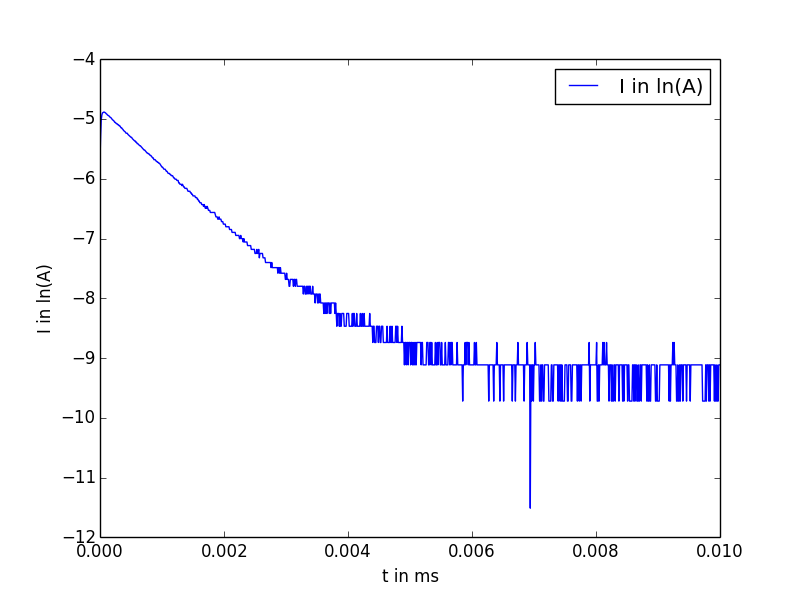
\includegraphics[scale=0.35]{ln(I)ggt.png}\\
Logarithmierter I-Datensatz (Einheiten siehe Grafik)\\
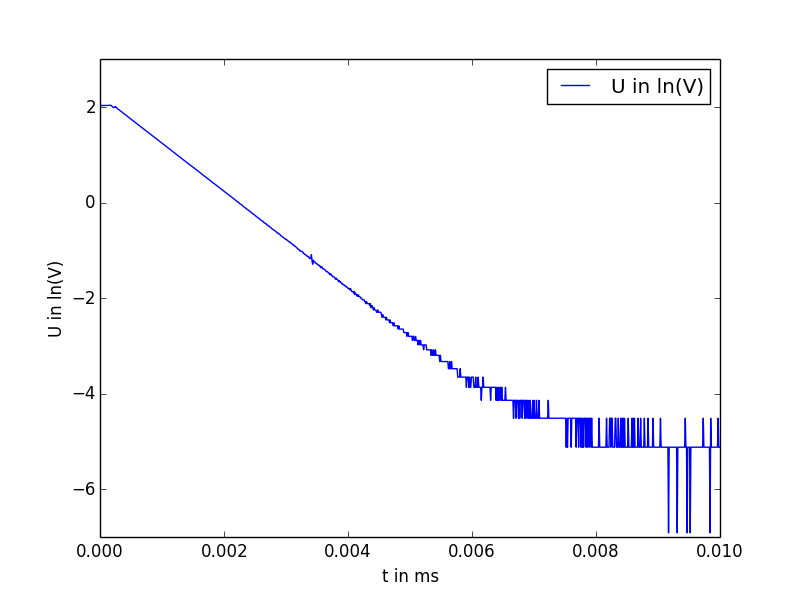
\includegraphics[scale=0.35]{ln(u)ggt.png}\\
Logarithmierter U-Datensatz (Einheiten siehe Grafik)\\
\\ Wir erkennen eindeutig am Anfang und Ende unserer Daten Bereiche, die in einer lineare Regression unser Ergebnis deutlich verfälschen würden. Wir werden daher nur Datenpunkte nehmen, die einer Geraden auf der logarithmischen Skala entsprechen.
Nun sehen unsere Daten wie folgt aus:\\
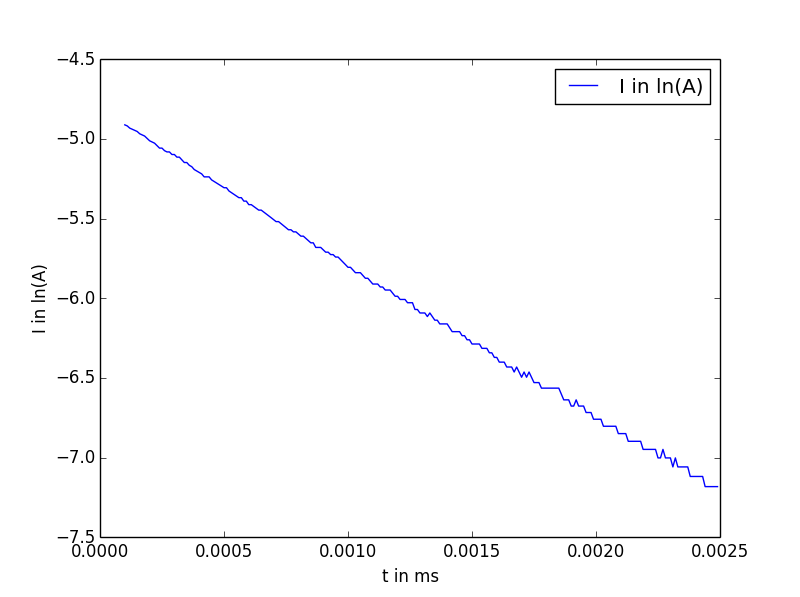
\includegraphics[scale=0.35]{ln(Ik)ggt.png}\\
Logarithmierter I-Datensatz mit angepasstem Bereich(Einheiten siehe Grafik)\\
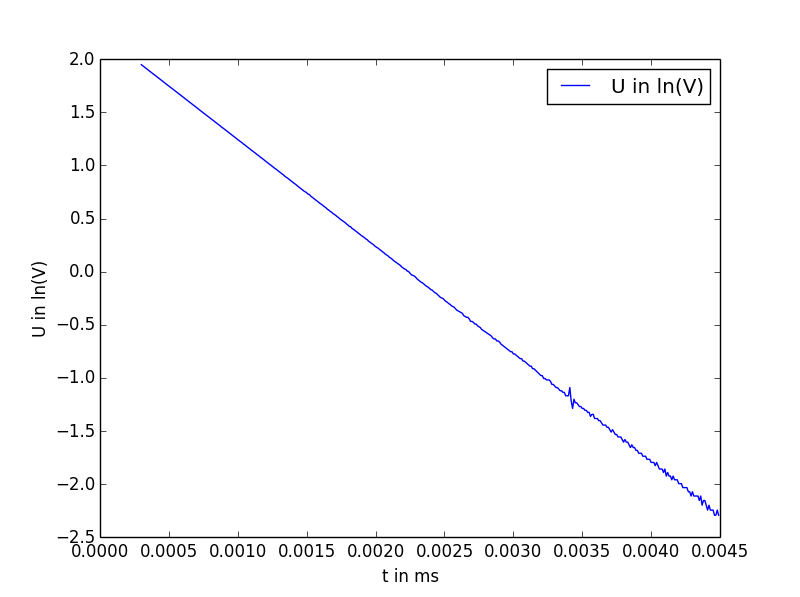
\includegraphics[scale=0.35]{ln(uk)ggt.png}\\
Logarithmierter U-Datensatz mit angepasstem Bereich(Einheiten siehe Grafik)\\
\\Jetzt führen wir die Lineare Regression durch.\\
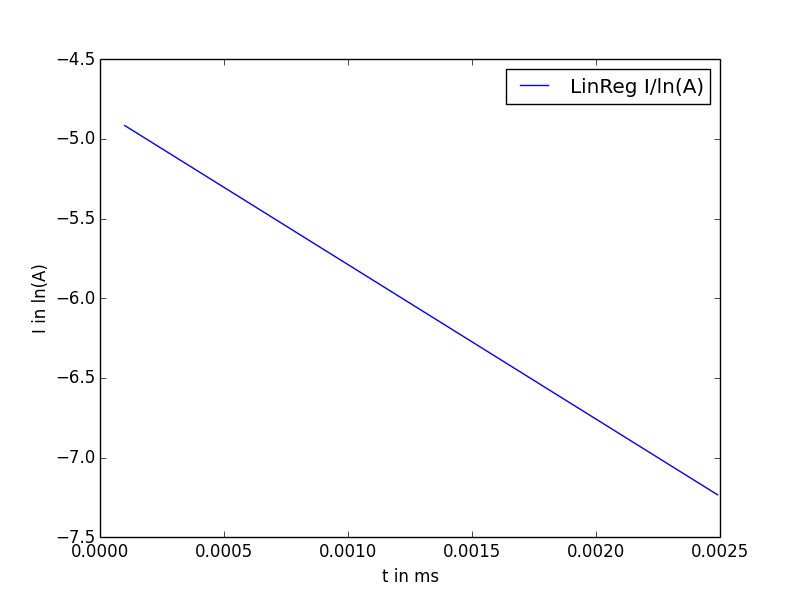
\includegraphics[scale=0.35]{lin_reg_I}\\
\\$\chi^2 = 3.046431$\\
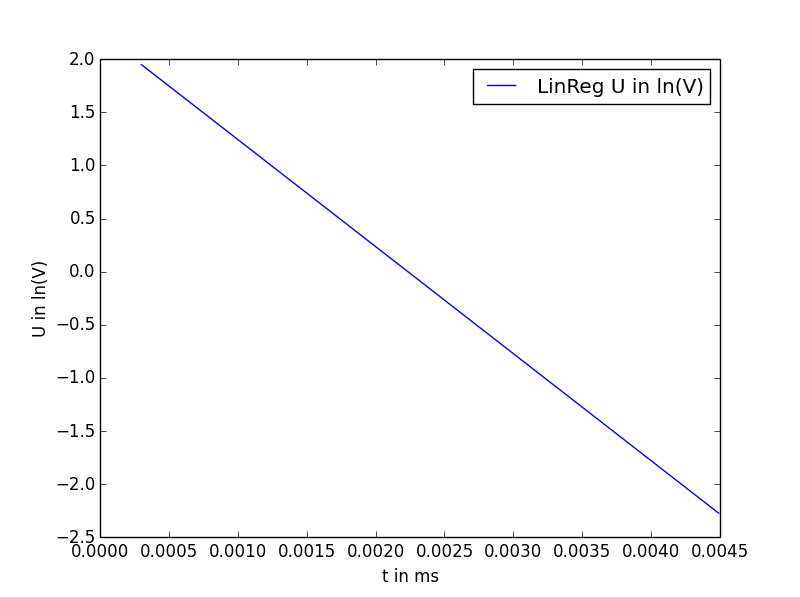
\includegraphics[scale=0.35]{lin_reg_U}\\
\\$\chi^2 = 2.469800$\\
\\Der Fehler pflanzt sich wie folgt fort:\\
\\$\sigma_{LinReg} = \frac{\sigma_I}{I}$\\
\\Um die Unsicherheit auf U zu bestimmen verfahren wir genauso wie bei I.\\
Die Lineare Regression hat die Form a$\cdot x + $b. Wie im Skript erläutert können wir nun aus unserem vorher bestimmten Widerstand (siehe Versuch 1) und der Steigung der Geraden die Kapazität ausrechnen.\\
\\$C = -\frac{1}{a\cdot R}$\\
\\Daraus ergibt sich die statistische Unsicherheit auf C von:\\
\\$\sigma_C = \sqrt{(\frac{\sigma_a}{a})^2+(\frac{\sigma_R}{R})^2}\cdot C$\\
\\Wir prüfen anhand der Residuenverteilungen, ob die Offset-Korrektur ausreichend war. Das Residuum erhalten wir, indem wir die Differenz von unseren Daten und dem Fit bilden. Die Fehler werden wie üblich fortgepflanzt.\\
\\$Residuum = I - LinReg(I)$\\
Analog dazu U.\\
\\$\sigma_{Residuum} = \sqrt{(\sigma_{I})^2+(\sigma_{LinReg})^2}$\\
Das sollte uns gleichverteilte Werte als Streuung um 0 zurückgeben.\\
\includegraphics[scale=0.35]{residuum_I}\\
Residuum für I 
\includegraphics[scale=0.35]{residuum_U}\\
Residuum für U
\\Man erkennt eine $sin^2$-Systematik im Residuum für I, dies führen wir auf unsere unstete Spannungsquelle zurück. In den unbearbeiteten Cassy-Daten sieht man, dass sich die Spannungsquelle unregelmäßig an- und ausstellt. Das Residuum für U ist größtenteils gleichverteilt, streut aber am Ende auch mit einer $sin^2$ Charakteristik. Unser $\chi^2$ von 3.0 bzw 2,5 ist allerdings zufriedenstellend.\\
\\Danach pflanzen wir den systematischen Fehler fort:\\
\\$\sigma_{c_{sys}} = \frac{1}{a\cdot R^2}\cdot\sigma_{R_{sys}}$\\
\\Danach wiederholen wir alles für die restlichen Messungen und bilden den gewichteten Mittelwert:\\
\\$\bar{C} = \frac{\sum{\frac{C}{(\sigma_{sys}+\sigma_{stat})^2}}}{\sum{\frac{1}{(\sigma_{sys}+\sigma_{stat})^2}}}$ und $\sigma_{C_{ges}} = \sqrt{\frac{1}{\sum{\frac{1}{(\sigma_{sys}+\sigma_{stat})^2}}}}$\\
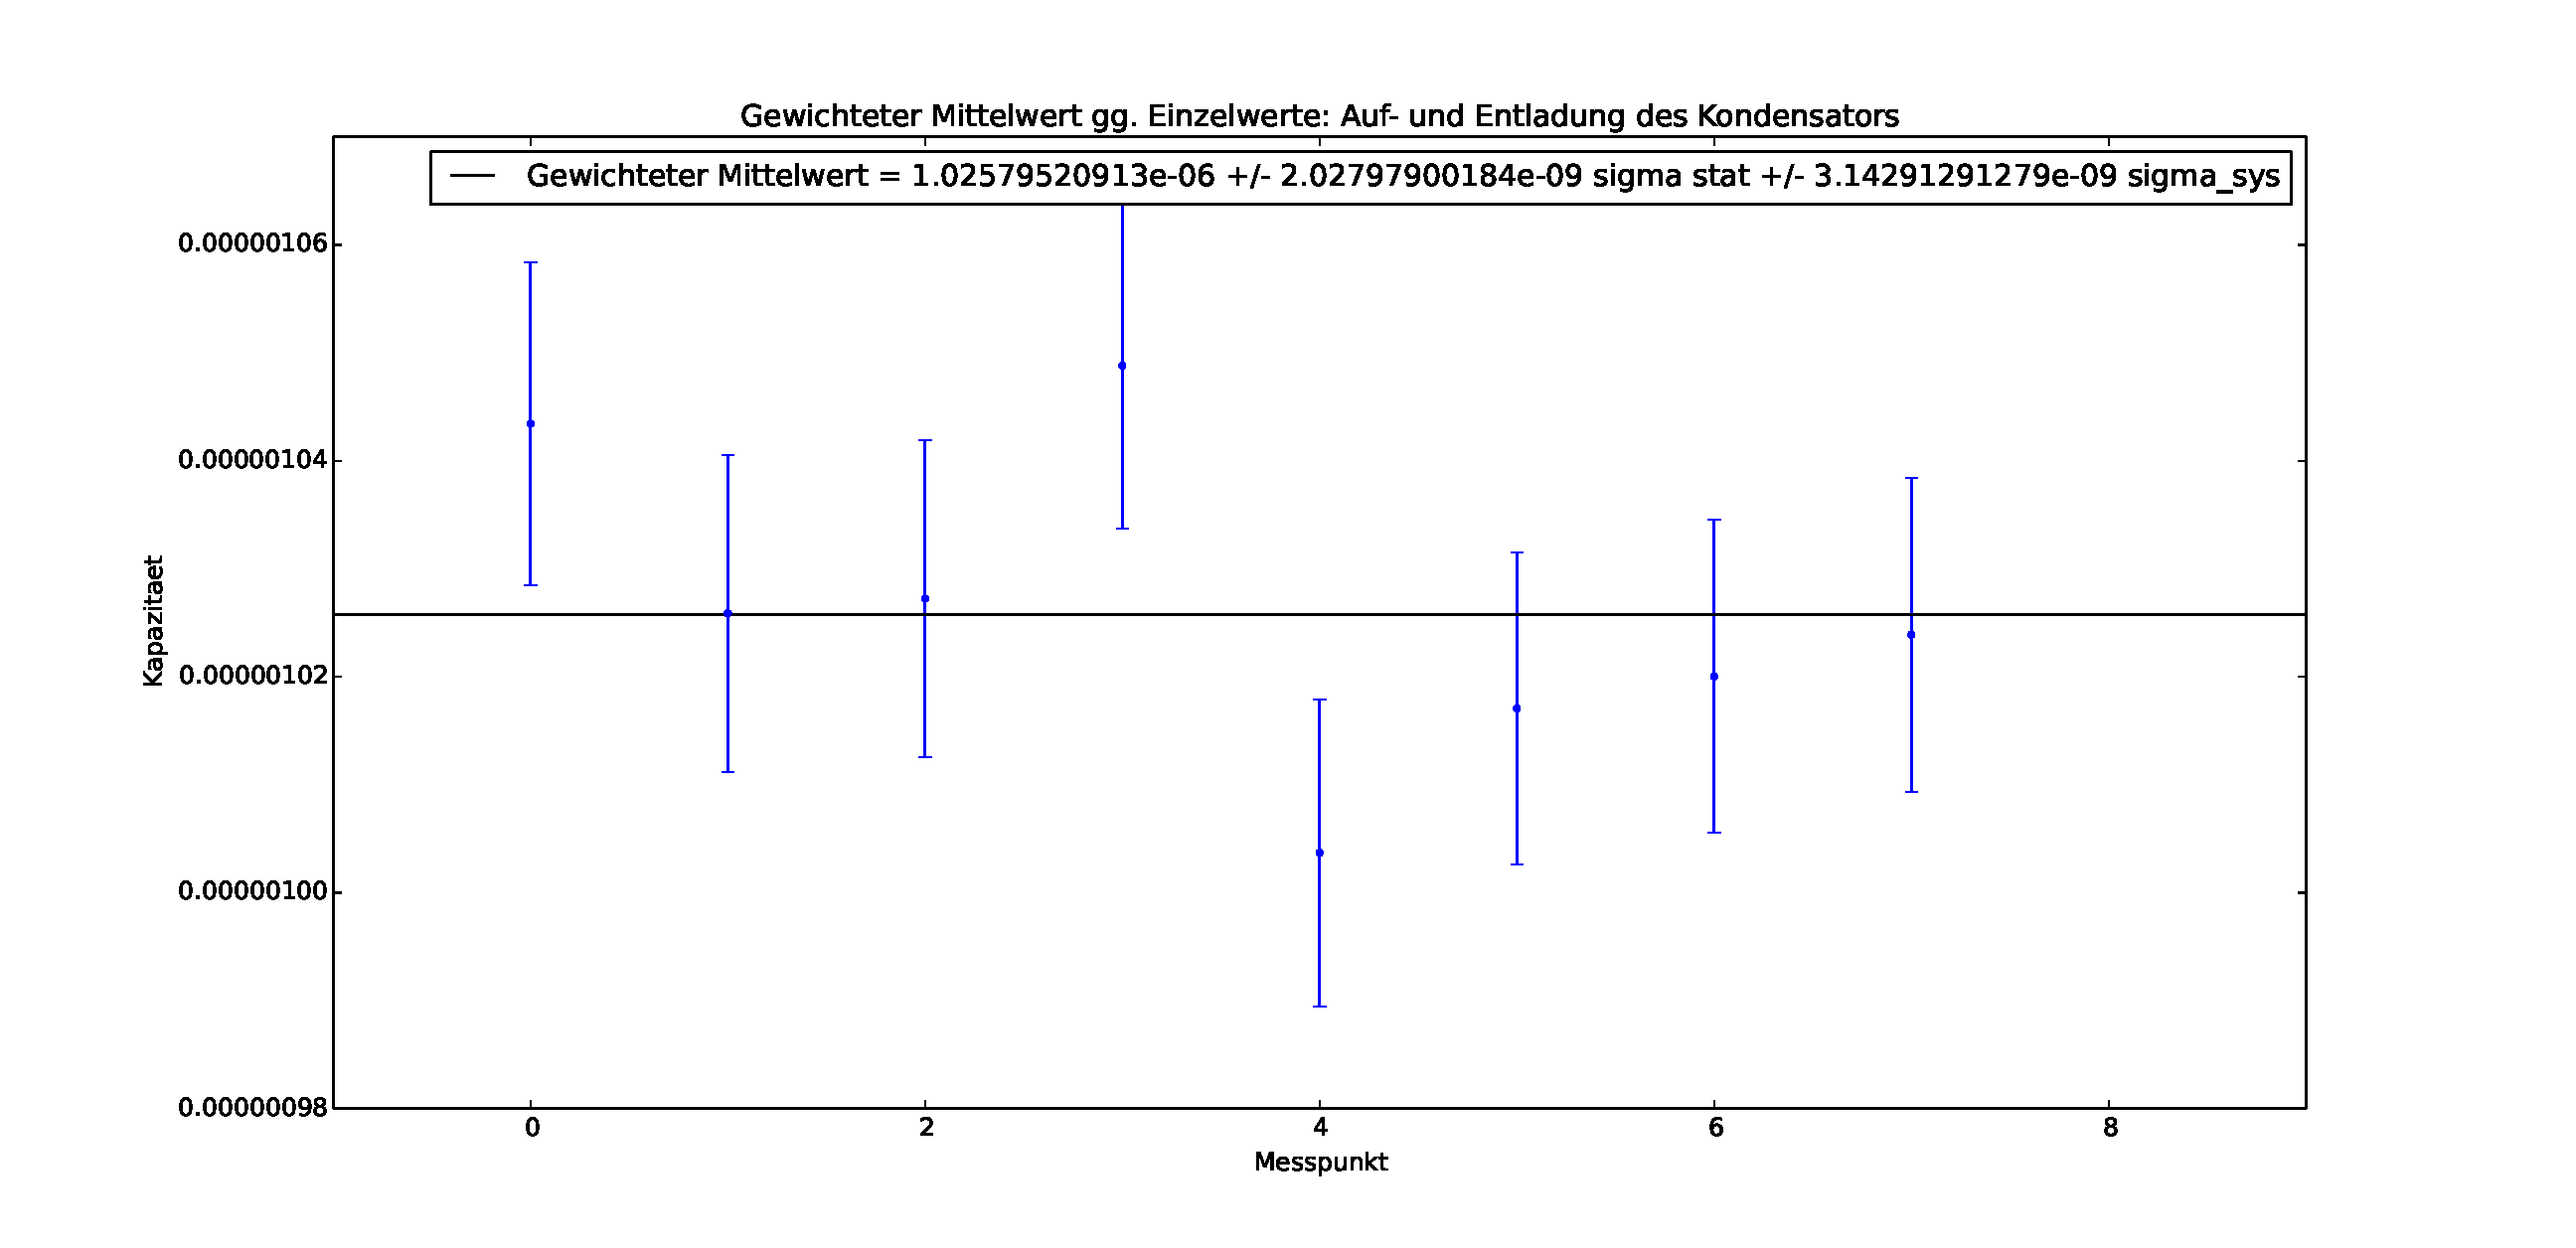
\includegraphics[scale=0.4]{verteilung_mean.eps}\\
\\Die Streuung der Einzelwerte um den gewichteten Mittelwert liegt zu ca 60\% im Rahmen der Unsicherheit auf die Einzelmessungen. Wir sind mit diesem Ergebnis sehr zufrieden.\\
\\Wir erhalten für unseren Kondensator einen Wert von: C = 1.026$\mu F \pm$ 2.028$\cdot 10^{-3}\mu F \pm$3.143$\cdot 10^{-3}\mu F$. 

\subsubsection{Fazit}
Unser Wert für C liegt mit 1.026 $\mu F$ innerhalb der 5\% Toleranzgrenze des Herstellers (0.95$\mu F$-1.05$\mu F$), unser $\chi^2$ liegt in einem zufriedenstellenden Bereich und der Wert stimmt auch mit der Vermessung des Kondensators mit der Greenbox überein (0.999$\mu F \pm$0,25\%).\\
\end{document}